\documentclass[a4paper,12pt]{article}
\usepackage[utf8]{inputenc}
\usepackage{graphicx}
\graphicspath{ {images/} }
\usepackage{amsmath}
\usepackage{tabularx}
\usepackage{latexsym}
\usepackage{amssymb}
\usepackage{bbm}
\usepackage{mathtools}
\usepackage[linesnumbered,ruled,vlined]{algorithm2e}
\usepackage{algpseudocode}
\usepackage{pifont}
\usepackage{float}
\usepackage[margin=1.2in]{geometry}
\DeclarePairedDelimiter\ceil{\lceil}{\rceil}
\DeclarePairedDelimiter\floor{\lfloor}{Q\rfloor}

\title{Mathematical Optimization in Database Systems: Deterministic and stochastic ILPs}
\author{Ahmad Chatha}

\SetKwInput{KwInput}{Input}                % Set the Input
\SetKwInput{KwOutput}{Output}              % set the Output

\begin{document}

\maketitle

\begin{abstract}
\begin{quote}
Mathematical optimization has gained traction in various fields in the recent years. Traditional Database systems have somewhat lagged behind in incorporating constrained optimization into their query execution workflow and instead rely upon the conventional optimization techniques. However, many practical, real-world queries can be expressed as a constrained optimization problems and it makes sense to provide in-database support of solving these problems directly from the database queries. This involves not only coming up with a language that supports expressing these optimization constraints but also solving the optimization problem and returning results all from within the database. This paper explores the use of mathematical optimization in database systems by investigating Package queries in Relational databases and their stochastic version [1, 2]. Package queries rely on Integer linear programming (ILP) as a black-box system to execute queries that require a collection of result tuples that satisfy a set of constraints while optimizing some cost function. Also, we try to approximate the ILP using a linear program (LP) and see whether it affects the performance and quality of results. The code is available on github.\footnote{https://github.com/ahmadchatha/Scalable-PaQL-Queries}
\end{quote}
\end{abstract}
\vspace{5mm}
\\

\\\\
{\large\textbf{1. Introduction}}
\vspace{5mm}

Optimization problems arise in many different fields such as automatic control systems, estimation and signal processing, communications and networks, electronic circuit design, data analysis and modeling,
statistics, and finance. A typical workflow, in solving such problems, involves extracting the data from a database, processing it, formulating and running the optimization problem using a solver and then perhaps storing the results back in the database. Following are some examples of real-world scenarios that result in optimization problems we are interested in.
\\

{\small Example 1 (Allocation/Scheduling): \textit{Given a set of machines with their costs and availability; a set of jobs to be done, each consuming a specified amount of resources and the returns for each job, the problem is to determine how much of each resource to allocate to each job while minimizing the cost and maximizing the returns from the jobs.}\par}
\vspace{5mm}
{\small Example 2 (Routing): \textit{Given a set of nodes and the paths between them along with the time, cost and distance for traversing those path, the problem is to find an optimum route between two or more nodes while keeping the cost, time and distance as low as possible.}\par}
\vspace{5mm}

{\small Example 3 (Financial Portfolio):\textit{Given uncertain predictions for future stock prices based on financial models derived from historical data, an investor wants to invest \$1,000 in a set of trades (decisions on which stocks to buy and when to sell them) that will maximize the expected future gain, while ensuring that the loss (if any) will be lower than \$10 with probability at least 95\%.}[1]\par}
\vspace{5mm}

The data these problems require is often housed in a traditional database systems. Therefore, it makes sense to implement the optimization problem within the database and present end users with an intuitive sql-like language they can use to execute queries like these. These queries operate on collection of tuples instead of individual records in the database. These tuples have to collectively satisfy global and local constraints in order to be included in the result. When the data is known, these queries are deterministic in nature (PaQL)[1] and for unknown attributes they are stochastic (sPaQL) [2].
\\

1. {\small \textbf{Deterministic Package Queries}}: Traditional databases rely on SQL as a query language to operate on individual records that satisfy a particular condition. When it comes to operating on multiple/group of records that satisfy given constrains collectively, SQL ends up involving complex self-joins or recursion. This not only affects readability of these queries but also the performance as the result set explodes. PaQL aims to extend SQL by adding minimal changes in order to maintain readability and still able to run queries on collection of tuples. Because these queries are of combinatorial nature, they are not solvable by the traditional database system. These package queries are, instead, converted to integer linear programs which are solved by an external optimization solver. There is a one-to-one correspondence between a package query and an ILP. Since an integer linear program is NP-Hard, the package queries are also NP-hard as a result. Solving an ILP on the entire dataset can be rather slow. Instead, the dataset is partitioned and ILP is run on small subsets of data which are continuously refined along the way to arrive at the final answer. This approach is called \textit{SketchRefine} [1].
\\

2. \textbf{Stochastic Package Queries}: These queries are much like their deterministic counterpart, except that the data they operate on is of stochastic nature and is uncertain. The uncertainty is modeled through some complex distribution such as log-normal variates based on “geometric Brownian motion” [3]. Stochastic Package queries (SPQs) use Monte Carlo probabilistic data model to generate enough scenarios to model the uncertainty in data [2]. The stochastic integer linear program based on these scenarios is then approximated by a deterministic ILP (much like the case in PaQL) and the solution is validated afterwards. If its infeasible then more scenarios and generated and the process is repeated. The large amount of data requires a huge number of scenarios and as a result the ILP solver mostly fails. In order to get around that problem, the large set of scenarios is replaced by a well-representative "summary" of the scenarios and this reduced set is then passed to the ILP solver resulting in \textitP{SummarySearch} algorithm [2].
\\

Section 2 lists some related systems that are similar to Package queries. Section 3 takes a deep dive into (s)PaQL. Section 4 shows its correspondence to an integer linear program. Section 5 contains details about the SketchRefine algorithm. Section 6 contains details about SummarySearch. Section 7 presents some experiments, results and Discussion. Section 8 lists some future directions. Finally, we conclude with Section 9.

\vspace{5mm}
\textbf{2. Previous Work}
\\

Package queries are related to systems where we apply constraints to a set of tuples while minimizing or maximizing a certain objective function. There are various set-based recommendation and scheduling systems out there that try to apply constraints on a set of tuples. For example, CourseRank [4] tries to recommend courses to students in universities that satisfy given constraints such as scheduling conflicts, pre-requisites, etc. These systems usually have their own ad-hoc query languages. These queries can be expressed as PaQL but the opposite may not be true.
\\
Another system that closely resembles PaQL is Tiresias [5]. Tiresias tries to answer the queries of the form "How-to" change the input in order for the output to meet a specified criteria. In that sense, it answer the hypothetical what-if questions. Similar to PaQL, the problem instance is transformed into an Integer linear program which is solved by an external solver. Everything sits on top of a relational database as is the case with PaQL. In order to solve the ILP problems faster, divide and conquer strategy is used to break the problem instance into small pieces. However the query language is not as nice as that of PaQL. Instead of using SQL they use a variant of Datalog which can be extremely verbose as shown in Figure 1. Package queries look much simpler and a lot like an optimization problem. Moreover TiQL works on the datasets while PaQL works with a collection of tuples. PaQl allows repetitions in result whereas TiQL does not. \\
\begin{figure}[h]
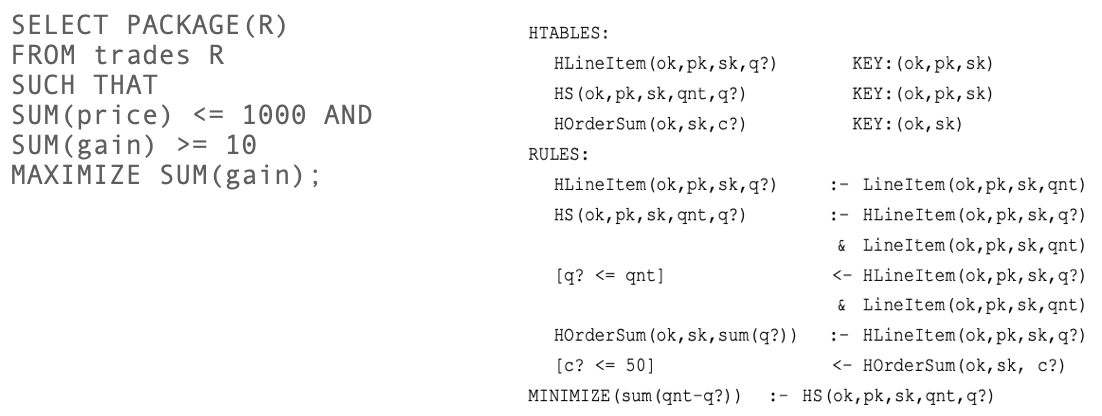
\includegraphics[scale=.7]{1}
\caption{Comparing the structure of a PaQL query on the left with a datalog based TiQL query that on the right[5]. Both use a black-box optimization solver to find a feasible solution to the queries.}
\centering
\end{figure}
\\
SolveDB [6] is another system which tries to integrate Optimization solvers into SQL Databases.  It comes with its own pre-installed solvers including linear programming, mixed-integer programming, global black-box optimization, and domain specific problems. It uses a so-called \textit{solve-query} language which is based on SQL-like syntax. An example query is shown in Figure 2 where a LP program is stated in solve-query as well as PaQL. It uses multiple select statement to gather all the data and perform the optimization in SolveDB where as PaQL syntax is much more concise. The constraints and the object function is neatly integrated with the single SQL SELECT statement. Unlike how PaQL uses SketchRefine to make the ILP run faster, SolveDB does not do any optimizations and leaves it to the solver to find a feasible solution.

\begin{figure}[h]
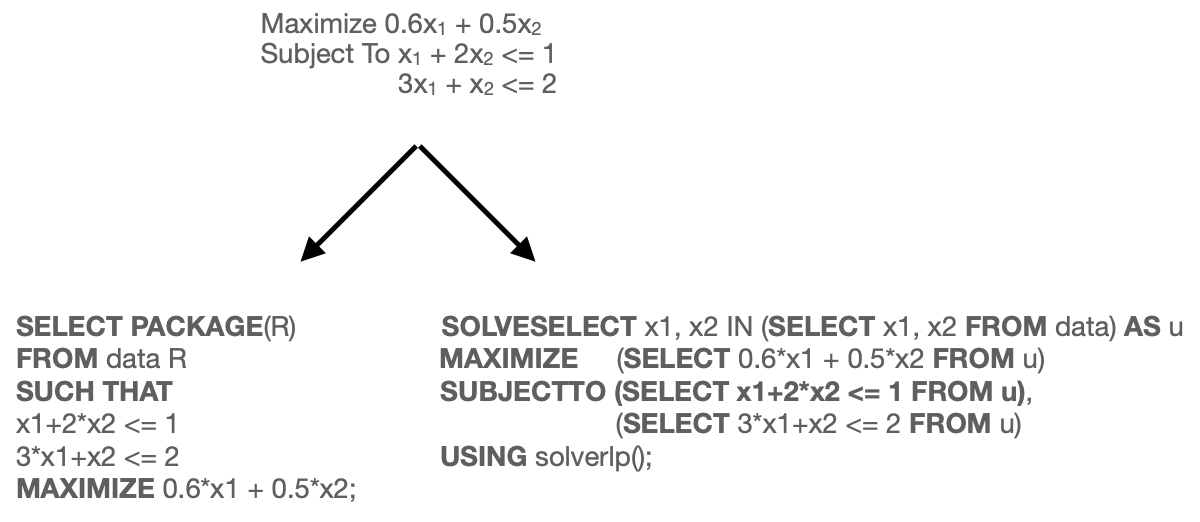
\includegraphics[scale=.7]{2}
\caption{A LP is converted to PaQL on the left and \textit{solve-query} format [6] on the right.}
\centering
\end{figure}

\\
Besides such similar systems, there is an extensive body of research in the field of Mathematical optimization field itself. There are various solvers out there that are getting improved everyday. PaQL relies on IMB's CPLEX solver but it can technically support any solver since it uses CPLEX as a black-box system. Moreover, the problem of ILP itself can be approximated in several ways. One approach is to use LP instead of ILP and then use rounding techniques [7]. One can also solve the ILP using the \textit{primal-dual method} too [8]. Techniques like these can be easily integrated into Package queries as minimal assumptions are made as to how the solver comes up with an answer. The Stochastic version could also benefit from the advances being made in Stochastic optimization. 
\vspace{5mm}
\\\\
\textbf{3. (s)PaQL: The Package Query Language}

Anyone coming from a relational database environment should feel right at home with PaQL since it is just an extension to SQL language. It adds the ability to state optimizations problems on top of relational tables in a simple and intuitive way. In order to see the difference between a regular SQL query, a package query and its stochastic version, consider the PaQL query from Figure 1. We have a table of trades as shown below:
\\

\begin{tabularx}{.982\textwidth} { |p{2cm}|p{2cm}|p{2cm}|p{2cm}|p{2cm}|p{2cm}| }
 \hline
 \textbf{id} & \textbf{stock} & \textbf{price} & \textbf{sell-in (days)} & \textbf{gain} & \textbf{category} \\
 \hline
1  & NVDA  & 302 & 1 & 3 & tech \\
\hline
2  & NVDA  & 302 & 7 & 25 & tech\\
\hline
3  & NVDA  & 302 & 10 & -20 & tech \\
\hline
4  & PYPL  & 183 & 1 & 6 & tech\\
\hline
5  & PYPL  & 183 & 2 & 10 & tech\\
\hline
6  & AMZN  & 768 & 1 & 200 & tech\\
\hline
7  & AMZN  & 768 & 3 & -200 & tech\\
\hline
8  & AMZN  & 768 & 7 & 400 & tech\\
\hline
9  & AMZN  & 768 & 15 & -500 & tech\\
\hline
\end{tabularx}
\\

We want to find set of trades that give us the best gain/return satisfying price $<= 1000$, gain $>= 10$ and category = 'tech' constraints. A quick glance will give us the result manually and its 410 with ids 5 and 8. Following are the regular sql and PaQL queries for comparison:
\\
\begin{figure}[h]
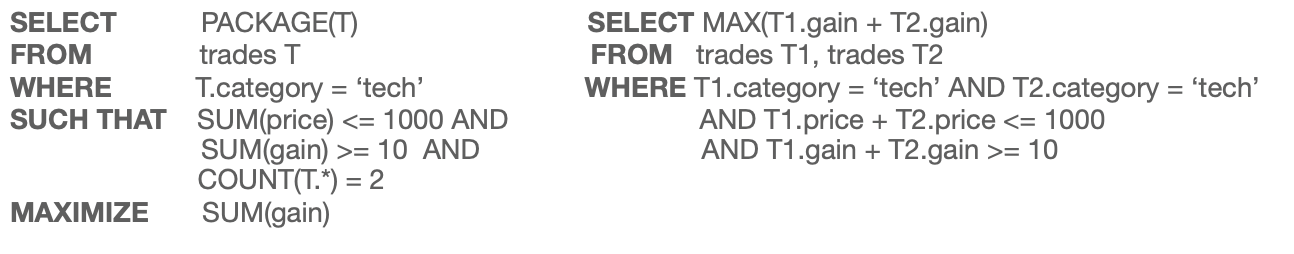
\includegraphics[scale=.7]{3}
\caption{PaQL on the left and an equivalent regular SQL query on the right.}
\centering
\end{figure}

As written, the two queries are computing the same result. But if we remove the constraint \textbf{COUNT(T.*) = 2}, the PaQL query becomes much more powerful as it will find you any number of rows that maximize the gain. For this particular small dataset the optimal solution happens to involve only 2 rows (5 and 8) and hence the regular SQL query has two self joins. If the results were to involve more than two rows then we would need the equivalent number of self-joins which can become cumbersome to say the least. PaQL, however, does not depend on the number of tuples in the result set since it scales as written.
\\

Of course, this query only works on historical data where \textbf{gain} is known already. What if we want to run the query on data where we don't know what the gain will be. That's where stochastic package queries come in. sPaQL is just an extension to PaQL and allows specification of package queries with stochastic constraints. The gain now becomes a random variable and therefore we maximizes the \textbf{EXPECTED} gain. We can also guarantee that the result is true with a certain probability with the keyword \textbf{PROBABILITY}. The query operates on \textbf{gain} data that is generated using the Monte Carlo probabilistic data model which allows us to define a VG (variable generation) function for each of the random variables. If we have more than one random variable then we can have an individual VG function for each one. These functions are called to generate \textit{enough} scenarios that are mutually independent and identically distributed (iid). The more the scenarios, the better the approximation.  The above query becomes:  

\\
\begin{figure}[h]
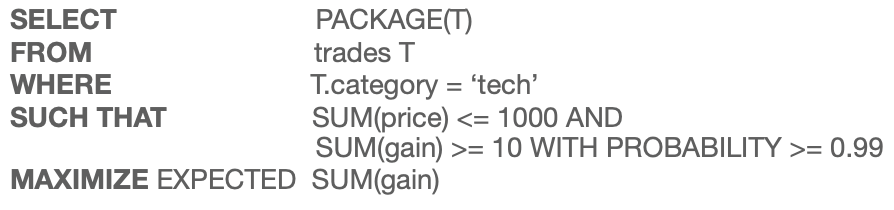
\includegraphics[scale=.7]{4}
\caption{Extension to PaQL to allow stochastic constraints.}
\centering
\end{figure}
\\
\vspace{5mm}

\textbf{4. PaQL $<=>$ ILP}
\\

Package queries are as hard as Integer liner programs. Since ILPs are NP-hard, so are Package queries.
\\

\\
{\small \textbf{Theorem 1}: \textit{ Every integer linear program can be expressed as a package query [1].}\par}

Proof: The proof is based on reduction technique. We create a mapping from a generic ILP to a specific database instance and a PaQL query. Another mapping is created form a PaQL query to ILP. These mapping are created such that a feasible solution to ILP is also a feasible solution for PaQL and the other way around. Let $\mathcal{L}$ be the following generic instance of an ILP:
\\
\begin{gather}
    max \sum_{i=1}^{n} a_i x_i \\
    s.t \sum_{i=1}^{n} b_{ij} x_i \leq c_j \qquad   \forall j = 1,...,k \\
        x_i \geq 0, \quad x_i \in \mathbb{Z} \qquad   \forall i = 1,...,n
\end{gather}

To build a database instance $\mathcal{D}$ for $\mathcal{L}$ we build a relation R with attributes $1,...,k$ and an objective attribute. R contains n records $r_1, ..., r_n$ where each $r_i = (a_i, b_{i1}, b_{i2}, ... , b_{ik})$. The PaQL query associated with $\mathcal{L}$ is:
\\\\\\\\

{\large SELECT \space\space\space\space\space\space\space\space\space PACKAGE(R) AS P\par}
{\large FROM \space\space\space\space\space\space\space\space\space\space\space\space R \par}
{\large SUCH THAT \space\space\space SUM(P.$\text{attr}_j) \leq c_j$ \space\space $\forall j = 1,... ,k$ \par}
{\large MAXIMIZE \space\space\space\space\space SUM(P.$\text{attr}_{obj}$\par}
\\
\vspace{4mm}
Let $x$ be a solution for $\mathcal{L}$. The solution for Package P is constructed from $x$ by including each tuple $r_i$ exactly $x_i$ times.
\\

$(=>)$
If x is an optimal solution for $\mathcal{L}$, then p is an optimal package query for the database instance constructed. By construction:
\begin{gather}
\text{SUM(P.$\text{attr}_j$)} = \sum_{i=1}^{n} b_{ij} x_i \leq c_j \\
\text{SUM(P.$\text{attr}_{obj}$)} = \sum_{i=1}^{n} a_i x_i \quad \text{is maximal}
\end{gather}
\\
$(<=)$
if $p$ is an optimal package for query $\mathcal{Q}$ over the database instance then $x$ constructed from $p$ is an optimal solution for ILP instance $\mathcal{L}$. The proof is the same as the opposite direction above. $\square$

\vspace{5mm}
\textbf{5. SketchRefine: Solving a large ILP by solving smaller ILPs.}
\\

Since package queries are directly equivalent to ILPs we can evaluate them directly using ILP solvers. However, as the datasets become larger this becomes infeasible. Even with problems of smaller size, solvers like CPLEX have difficulty since they need the entire problem to fit in memory. Therefore, in practice, we are unable to solve the package queries due to their exponentially worst-case complexity even for small problems. SketchRefine [1] breaks the bigger ILP problem into smaller sub-problems which are solvable much faster. It does that by \textit{sketching} an initial package by only solving a much smaller ILP on a set of \textit{representative} tuples, which is much smaller than the original dataset. This is based on the intuition that \textit{similar tuples are likely to be interchangeable within packages} [1]. SketchRefine can be divided into three phases:
\\

\textit{5.1 Offline partitioning}
\\\\
Before the sketch and refine phase, we need to partition the data into similar groups of tuples in order to pick the representative tuple from each group for the sketch phase. We have two parameters in order to do the partition. A size parameter $s$ and a radius parameter $r$. We partition the dataset into $m$ groups until each group has size $\leq s$ and radius $\leq r$. The larger the size parameter $s$ the fewer the numbers of groups $m$. Generally we want to set $s$ in order to keep $m$ small for best response time. 
\\

There are many different ways to partition the dataset such as \textit{k-means} [9] or \textit{hierarchical clustering} [10] but they can't guarantee a partition size $s$ and radius $r$. Instead, SketchRefine uses k-dimentional quad-tree indexing [11]. The basic idea is to recursively partition the dataset into m groups by making sure that each group satisfies the size and radius constraints. We start by just having 1 group containing all the tuples. Since it has more than $s$ records, we partition it into $2^k$ where $k$ is the number of attributes in the relation table R. The group centroid is computed and used as a pivot to generate the new groups. This procedure is run recursively until we have $m$ groups satisfying group size and radius. The centroids chosen in the last step act as the representative tuples for the sketch process.
\\

It is important to note that the same partition can be used for many different queries workload. So we don't have to partition on the fly at the query time. Instead, we can do it offline in order to avoid the cost each time.  
\\\\
\textit{5.2 Sketch Phase}
\\

Given the representative tuples from the partitioning step, we produce a package query that is run directly by the ILP solver. Since this time we only have $m$ tuples there are only $m$ variables for the ILP problem to work with. If the solver is overwhelmed by the $m$ variables then we can further partition the dataset using the SketchRefine procedure itself recursively to further trim down the dataset and arrive at some number of representatives that can be efficiently handled by the solver directly. Note that there is a chance of producing a false negative. If the Sketch phase produces a query that is infeasible then the actual package may or may not be infeasible. However, the probability of this happening is low and bounded [1].
\\\\

\textit{5.3 Refine Phase}
\\

In this phase, we use the results of the sketch phase to arrive at a complete package containing the actual tuples from the original relation. This is done one group at a time. For each, group we derive a new package from the sketch package and replace the representative tuple with the actual tuples. The global constraints at this phase ensure that the tuples produced satisfy the original package query. Because each group size is $\leq s$ the ILP problem has only $s$ variable at most. Hence, we can solve the ILP directly via CPLEX solver. Just like the sketch phase, if the solver is over-whelmed, we can recurse using SketchRefine itself. 
\\

In theory, this phase only needs to refine each group one time. However, a refinement step for a particular group can make the query infeasible since the tuples are selected per group basis. It could happen that no other tuples form the remaining groups satisfy the constraints. In that case, SketchRefine resorts to a greedy backtracking approach [1]. The idea is to prioritize the group where the refinement query becomes infeasible, since this happened most likely due to the previous choices up until that point. The backtracking algorithm is run on a tree containing nodes representing unique sketch packages. Initially all the groups are placed on a priority queue. If an infeasible group is encountered we backtrack and put the group in front of the queue. If all the groups are infeasible, that means none of the groups could be refined and the query is infeasible. Otherwise if there aren't anymore groups to refine we return with a complete package.
\\

In the best case scenario, the algorithm never backtracks and all groups are feasible. We only make $\leq m$ calls to the ILP solver and each problem has $\leq s$ variables since the size of each group is at most $s$. In the worst case, we are never able to find a complete package as some group always ends up being infeasible. We make exponential number of calls to the ILP solver and the original package is declared infeasible. But, according to experiments, backtracking does not happen that often and usually we find groups that are feasible [1].
\\

It is important to note that the complete package produced by SketchRefine is approximate. It satisfies all the constraints of the original query but the object value may be sub-optimal. It is within certain approximation bounds [1] of the optimal value, however. Figure 5 below shows the three phases of SketchRefine [1]. 

\\
\begin{figure}[h]
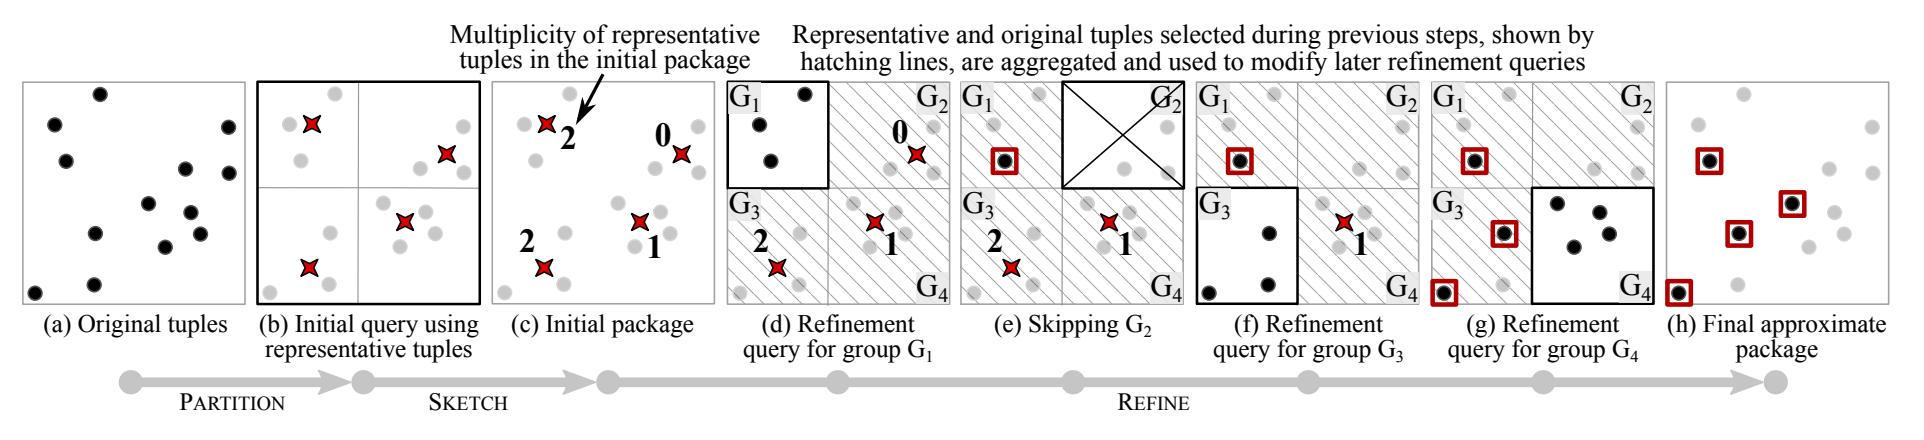
\includegraphics[scale=.5]{12}
\caption{Partitioning, Sketch and Refine steps of SketchRefine [1].}
\end{figure}
\\
\vspace{5mm}
\textbf{6. SummarySearch: Solving large SILP by solving smaller ILPs.}
\\

The Naive approach to solve the Stochastic integer linear program (SILP) involves generating scenarios using the Monte Carlo simulations. We then combines these scenarios into an approximate deterministic integer linear program. This is similar to the direct method in PaQL, but the deterministic ILP, itself, is only an approximation to the original SILP. This approach of solving a Stochastic ILP by approximating it with a deterministic one is called \textit{Sample Average Approximation} [12]. The deterministic ILP is solved by the CPLEX solver which gives us a solution $x$. Finally, this solution is validated against out-of-sample scenarios. Although simple, this approach fails in practice. The deterministic ILP becomes way too large for the solver to handle as it takes too many iterations of the optimize and validate phase. Moreover, even when it works, the problem takes too long to solve as the number of scenarios is usually too large. Lastly, there are no guarantees on the bounds of the optimal answer in relation to the original SILP.
\\

In order to get around the issues of the Naive approach, we need the size of the deterministic ILP to be much smaller. Instead of approximating the SILP using all the scenarios, we need to use as few as possible so that the solver can efficiently solve the much smaller deterministic ILP. This is what \textit{SummarySearch} [2] method tries to do by creating conservative \textit{summaries} of the entire set of scenarios. In many cases, the entire set is replaced by just 1 summary scenario. The result is that the approximated deterministic ILP size reduces a lot and we are able to use solvers like CPLEX efficiently. Moreover, SummarySearch provides approximation guarantees about the generated answer [2]. How these summaries are generated, how the approximation problem is formulated and the algorithm itself are described below:
\\

\textit{6.1 Generating Conservative Summaries}
\\

As before, we have a relation $R$ with $N$ tuples and with some uncertain attribute $A$. Without loss of generality, we can assume there is only one uncertain attribute $A$, though in practice we can have many such attributes. Assume that we have a set of $m$ scenarios $S = \{S_1, S_2, ... ,S_m\}$ which are just copies of relation $R$ with data generated for the uncertain attribute A. In order for a solution $x$ to be feasible for the approximated deterministic ILP, it has to satisfy a scenario $S_i \in S$ with respect to a probabilistic linear constraint of the form 
\[
    Pr(\sum_{i=1}^N t_iA x_i \bullet v) \geq p \tag{*}
\]
where $p \in [0,1]$, $\bullet \in \{\leq,\geq\}$, and $t_iA$ is the random variable according to attribute $A$ in tuple $t_i$. It changes to $s_{ij}A$ when its value is realized in scenario $S_j$. 
Then we define an $\alpha$-summary $S=\{s_iA : 1 \leq i \leq N\}$ based on the set of scenarios $S$ with respect to the $(*)$ constraint as a collection of N deterministic value of attribute $A$ such that if a solution $x$ satisfies S in $\sum_{i=1}^N s_iA x_i \bullet v$, then x satisfies at least $\ceil{\alpha M}$ of the scenarios set $S$ [2]. 
\\

A simple example of an $\alpha$ summary is a tuple-wise minimum or maximum over $\alpha$ scenarios out of $M$ scenarios. An example of an $\alpha$ summary on 4 scenarios of the relation R introduced in section 3 is shown in Figure 6 below. This summary is conservative in the sense that the gain of the summary is always less than the gain realized in any of the first three scenarios. So, if a solution $x$ satisfies the 0.75 summary, it will satisfy at least 0.75 of the $M$ scenarios. Larger the value of $\alpha$ the more conservative the summary is since it covers more scenarios. In some cases, it might satisfy $\geq \alpha$ scenarios. If it satisfy all $M$ scenarios than $x$ is feasible for the original problem. One can also come up with more sophisticated summary generation methods besides min and max.
\begin{figure}[h]
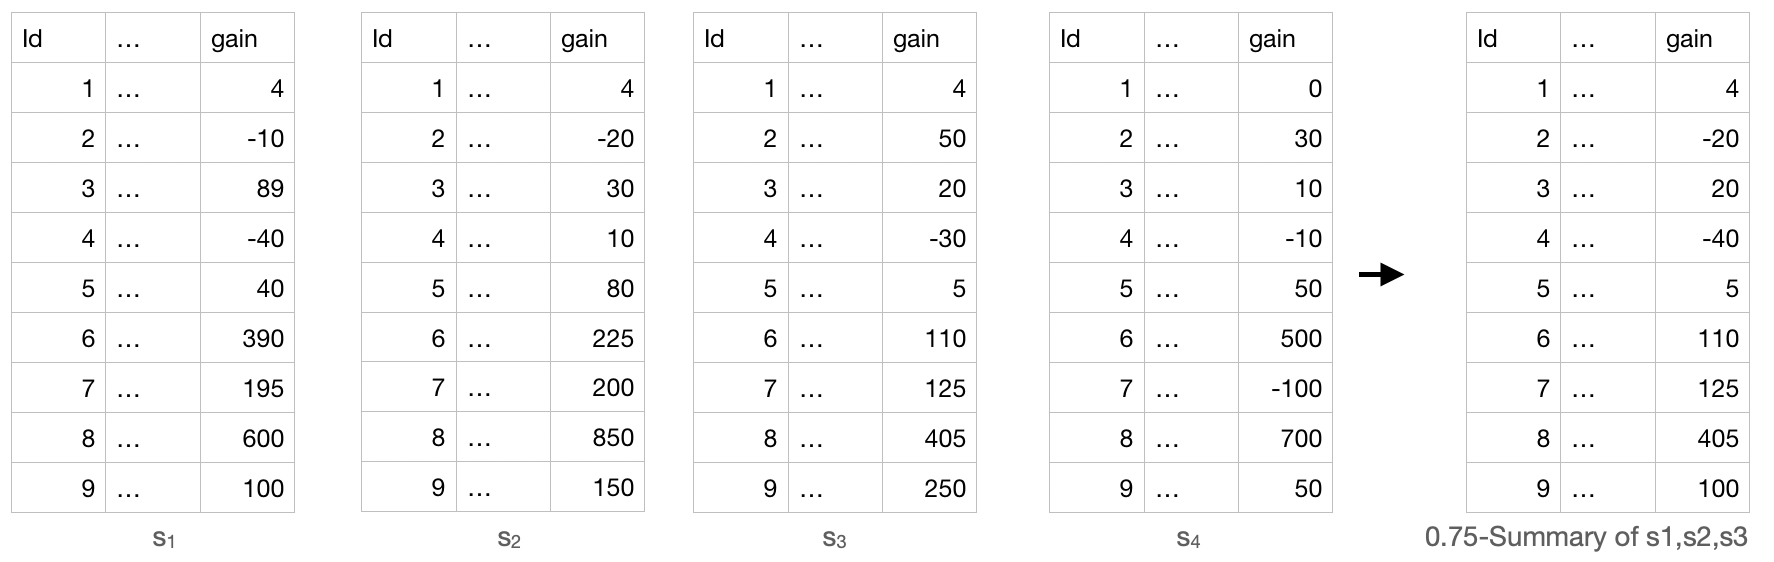
\includegraphics[scale=.5]{5}
\caption{Condensed form of Scenario 1, 2, 3, and 4 along with a 0.75 min Summary of scenario 1, 2, and 3.}
\centering
\end{figure}
\\

\textit{6.2 Formulating the Approximation problem based on the summaries}
\\

A solution $x$ to the approximated deterministic ILP in the Naive approach has to satisfy all the scenarios with respect the $K$ probabilistic constraints $(*)$ if $y_j = \mathbbm{1}(\sum_{i=1}^N s_{ij}A x_i \bullet v) = 1$ where $\mathbbm{1}$ is the indicator function (its 1 if $\sum_{i=1}^N s_{ij}A x_i \bullet v$ is true, 0 otherwise). Once we have the summaries, we can replace the scenarios and try to satisfy the constrainsts with the summaries instead. We have only talked about generating 1 summary for the $M$ scenarios. However, in general, we generate $Z$ summaries by randomly partitioning the scenario set S into $Z$ non-overlapping subsets. The $\alpha$ summaries are then generated from each of these $Z$ subsets. 
\\

For all the $K$ constraints of the form $(*)$, we add a new indicator constraint $y_z = \mathbbm{1}(\sum_{i=1}^N s_{iz}A x_i \bullet v)$ where $y_z \in \{0,1\}$. Solvers like CPLEX can handle these indicator constraints. A solution $x$ satisfies a summary $S_z$ if and only if $y_z=1$. To make sure, p\% of the summaries are satisfied we also add a linear constraint $\sum_{i=1}^Z y_z \geq \ceil{pZ}$.
\\

Note that if $Z=M$ then we only have 1 partition and the problem reduces to that of the Naive approach. In that sense, we can do at least as good as the Naive approach. However, in practice, Z is much smaller and the number of variables in the deterministic ILP is on the order of $(N \times Z \times K)$ where $N$ is the number of tuples, $Z$ is the number of summaries and $K$ is the number of the probabilistic constraints. In most cases, SummarySearch produces good results even when $Z=1$ [2].
\\

\textit{6.3 Query Evaluation and the Algorithm}
\\

Pseudo-code for SummarySearch algorithm is shown below[2]. The output is a feasible point $x$ with object value as close as possible to the object value of the deterministic ILP based on the $\hat{M}$ validation scenarios. On Line 1, we actually only solve a deterministic ILP since $\alpha = 0$ and none of the scenarios are required to be satisfied. If it has an infinite solution, then we simply ignore it and update $\alpha$ until a finite solution is found. This gives us the least conservative solution possible [2]. We start off with only 1 summary. On Line 6 we replace the actual $M$ scenarios with $Z$ summaries and solve the approximated deterministic ILP as shown above in 6.2 section. As long as we are not able to find a feasible solution, we increase $Z$ to improve optimality and increase $M$ to improve feasibility. If a feasible solution is found, we check whether the bounds are satisfied i.e. $\epsilon_x = (\omega_x - \hat{\omega})/\hat{\omega} \leq \epsilon$. SummarySearch takes a lot fewer iterations to find a feasible solution compared to the Naive approach [2]. The CSA-Solve [2] procedure can be found in the paper.
\\

\begin{algorithm}[H]
\DontPrintSemicolon
  
  \KwInput{\\Q: A Stochastic Package Query (SPQ) \\ 
           M: \# of scenarios\\
           Z: \# of summaries\\
           $\hat{M}$: \# of out-of-sample validation scenarios\\
           m, z: running iterates to M and Z respectively\\
           $\epsilon$: user defined error bound.}
  \KwOutput{a feasible point x or no solution}
  $x^{(0)} \xleftarrow{} Solve(SAA(Q_0, \hat{M}))$ \tcp*{probabilistically unconstrained problem}
  Z = 1   \tcp*{we start with 1 summary}
  x = null \tcp*{$x$ is solution for M}
  $\hat{v_x}$.is\textunderscore feasible = false \tcp*{$\hat{v_x}$ is solution for $\hat{M}$}
  \While {$\hat{v_x}$.is\textunderscore feasible is false and $\hat{v_x}$.upper\_bound $\geq \epsilon$}
  {
    $(x, \hat{v_x}) \xleftarrow{} $ CSA-Solve(Q, $x^{(0)}$, M, Z) \tcp*{Approximation based on the summaries.}
    
    set $\hat{v_x}$.is\textunderscore feasible based on validation
    
    \If {$\hat{v_x}$.is\textunderscore feasible and $Z \le M$}
    {
        $z\textprime \xleftarrow{} min\{z, M - z\}$
        $Z \xleftarrow{} Z + z\textprime$  \tcp*{increasing the \# of summaries}
    }
    \Else {
        $M \xleftarrow{} M + m$  \tcp*{increasing the \# of scenarios}
    }
  }

\caption{SummarySearch}
\end{algorithm}
\\
\vspace{5mm}
\textbf{7. Results \& Discussion}
\\
Results for ILP, SketchRefine, LP approximations and SummarySearch are described below. Results for PaQL and the LP approximations were generated based on the schema in section 3. Results for sPaQL are taken from the paper [2].
\\

\textit{7.1 PaQL (ILP v. SketchRefine v. LP)}
\\

We have the same schema as the example in section 3. The PaQL query used for the experiments is shown in Figure 7 below. We have four instances of the database with $N = 10; 100K; 1M; 10M $ records. The data was generated randomly with the script \textit{generate\textunderscore data.py} and loaded into a Postgres database. A Macbook with 16GB of RAM and 2.6 GHz 6-Core Intel Core i7 was used to run the experiments. For the blackbox ILP solver, IBM CPLEX version 12.6 was used. The data is first loaded from postgres into main memory and passed off to CPLEX. For SketchRefine, offline partitioning was performed by setting partition size threshold $s$ to be 10\% of the dataset size.  Most of the code was taken from the original paper [1]. Some tweaks were made to run these experiments and to generate the plots. Efforts were also made to compare regular SQL language, but they were unfruitful since it hopelessly breaks down even for a simple query as in Figure 7.
\\

The LP method is almost the same as the ILP method. The only different is that we don't restrict the solution to be integers i.e. $x \in \mathbb{Z}$. Instead we let $x$ to be continuous and round up to the nearest integer. The intuition is that the LP problem should be much easier to solve and should run faster while producing results that are close to the optimal value. Also, LP is not NP-hard whereas ILP is. 

\\
\begin{figure}[h]
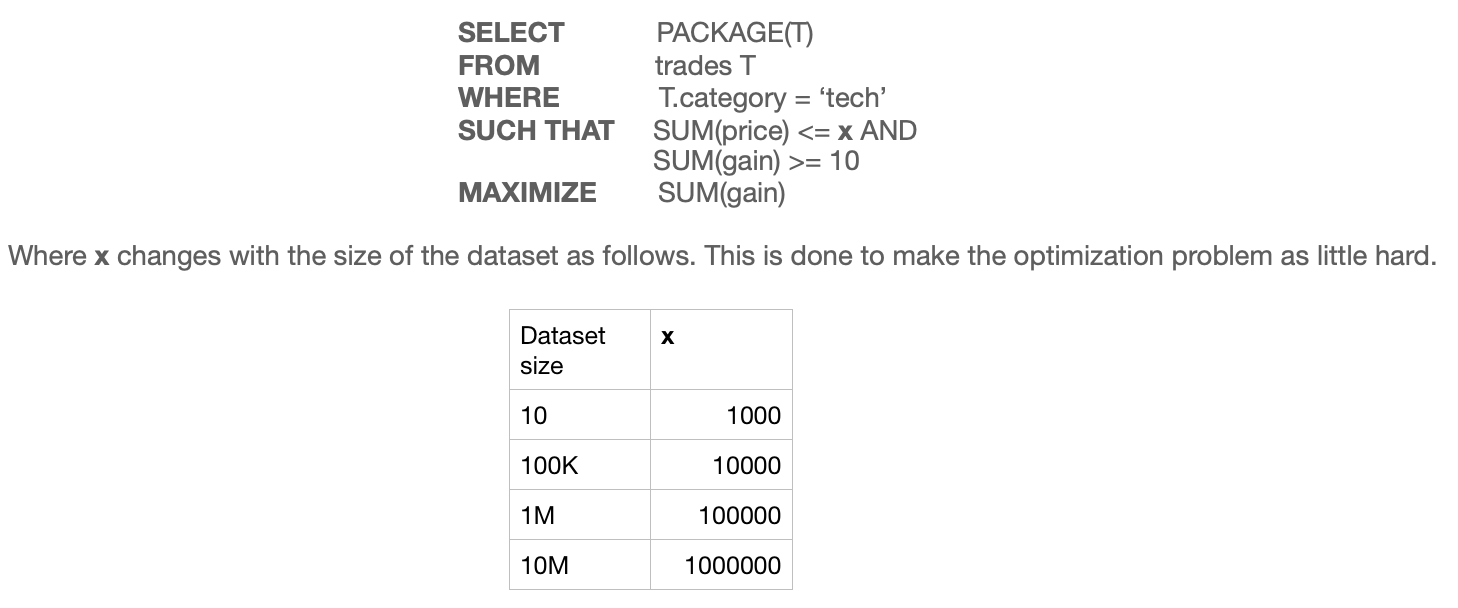
\includegraphics[scale=.6]{9}
\caption{PaQL query for DIRECT (ILP) v. SketchRefine v. LP }
\centering
\end{figure}
\\
Figure 8 below shows the times of all three methods as the size of the dataset is increased. The figure only shows the time spent in CPLEX optimization. As one can see, the direct ILP method takes the most amount of time, followed closely by the LP method. That was surprising and goes against our intuition. Both ILP and LP are similar problems and have the same # of optimization variables except the integer constraints. We suspect CPLEX just takes a fair amount of time processing all those variables because in theory LP is a much easier problem to solve. 
\\

SketchRefine, on the other hand, is much faster than both ILP and LP when it comes to the time spent optimizing. The reason for this difference is the fewer number of variables involved in the optimization problem. For both ILP and LP the number of variables scale with the size of the dataset. Whereas for SketchRefine, we solve ILP problems of much smaller size and fewer variables. Results for Direct (ILP) and SketchRefine corroborate with the findings in the paper as shown in Figure 8 below [1]. Note that SketchRefine still relies on ILP to solve its smaller problems and we did not do experiments replacing those smaller ILPs with LPs as there wasn't considerable difference between the times for LP and ILP.
\\\\\\

\begin{figure}[h]
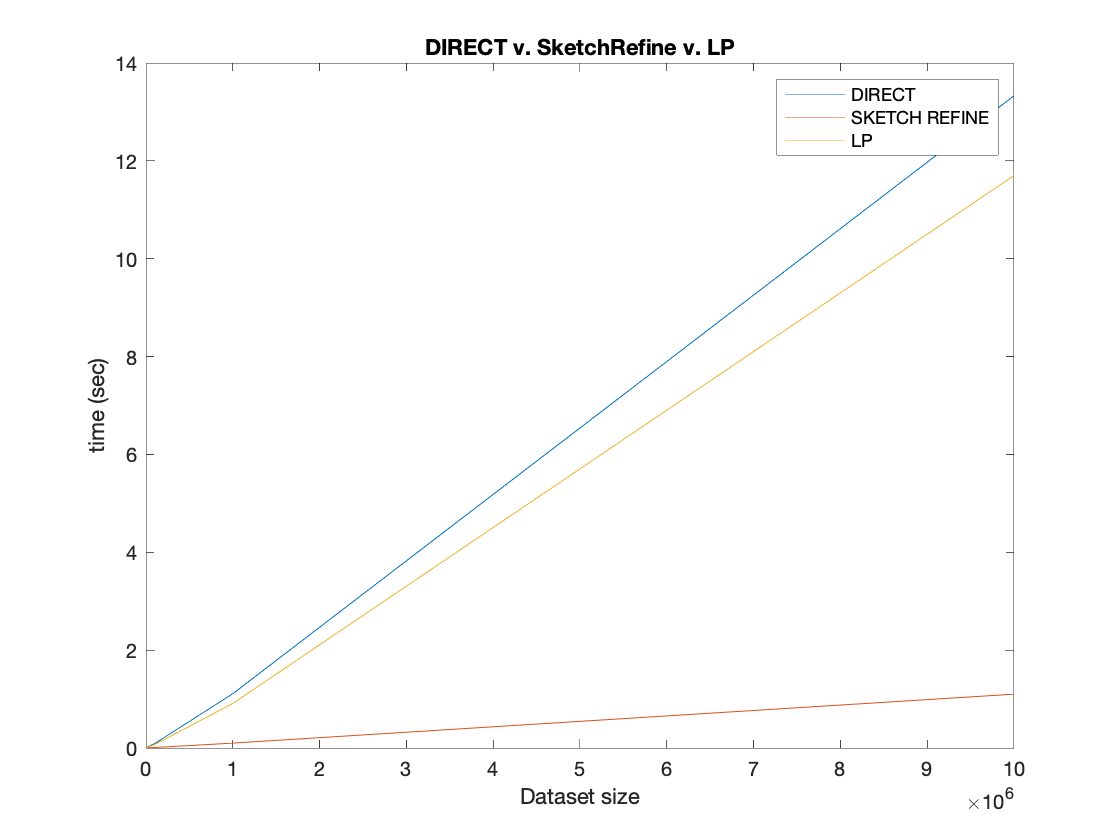
\includegraphics[scale=.4]{6.png}
\caption{DIRECT (ILP) v. SketchRefine v. LP (Optimization Response Time comparison).}
\centering
\end{figure}
\\
\begin{figure}[h]
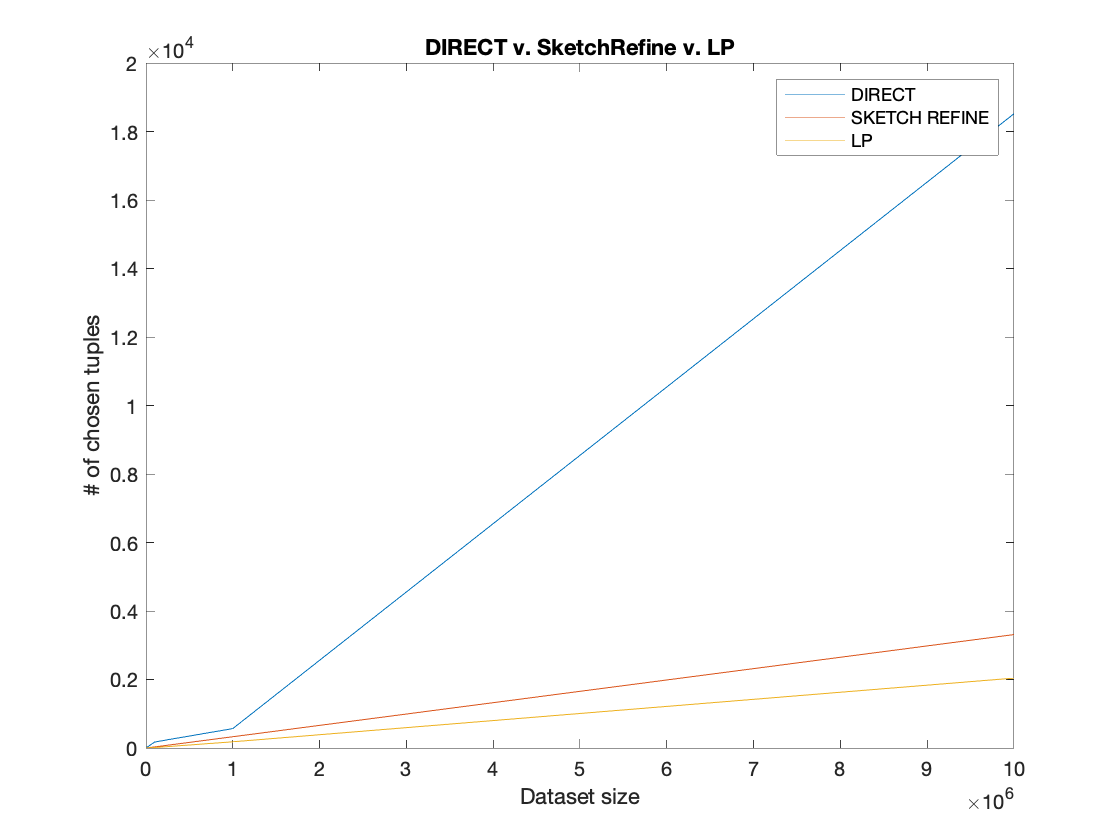
\includegraphics[scale=.4]{7.png}
\caption{DIRECT (ILP) v. SketchRefine v. LP (\# of tuples chosen).}
\centering
\end{figure}
\\

Figure 9 below shows that the number of tuples chosen increase as the size of dataset goes up. That makes sense because the price constraint goes up and we are allowed more money to purchase stocks. Interestingly, the size of feasible solution for LP contains the least amount of tuples because we chop off many solutions that don't make the rounding cut. SketchRefine which itself is an approximation to the ILP picks up more tuples than LP but it isn't very far. ILP, however, picks a lot of tuples that make up the objective value as compared to the other two approaches. As the dataset size goes up, there are many candidates that give us the optimal value. It seems that ILP is finding a lot of tuples that give us smaller gain to maximize the profit. LP and SketchRefine, on the other hand, tend to pick tuples with large gains and as a result end up with fewer tuples that make up the objective value.
\\

Figure 10 shows the objective value for the three approaches. The graph shows no distinguishable difference between the three methods. We already know from the PaQL paper [1] that SketchRefine's solution is bounded and very close to the Direct (ILP) approach. Surprisingly, LP is also very close to the optimal value. Its within 99\% of the optimal value for our experiments. However, query performance for LP, while better than ILP, isn't as good as SketchRefine which is about an order of magnitude faster than both ILP and LP. 
\\
\begin{figure}[h]
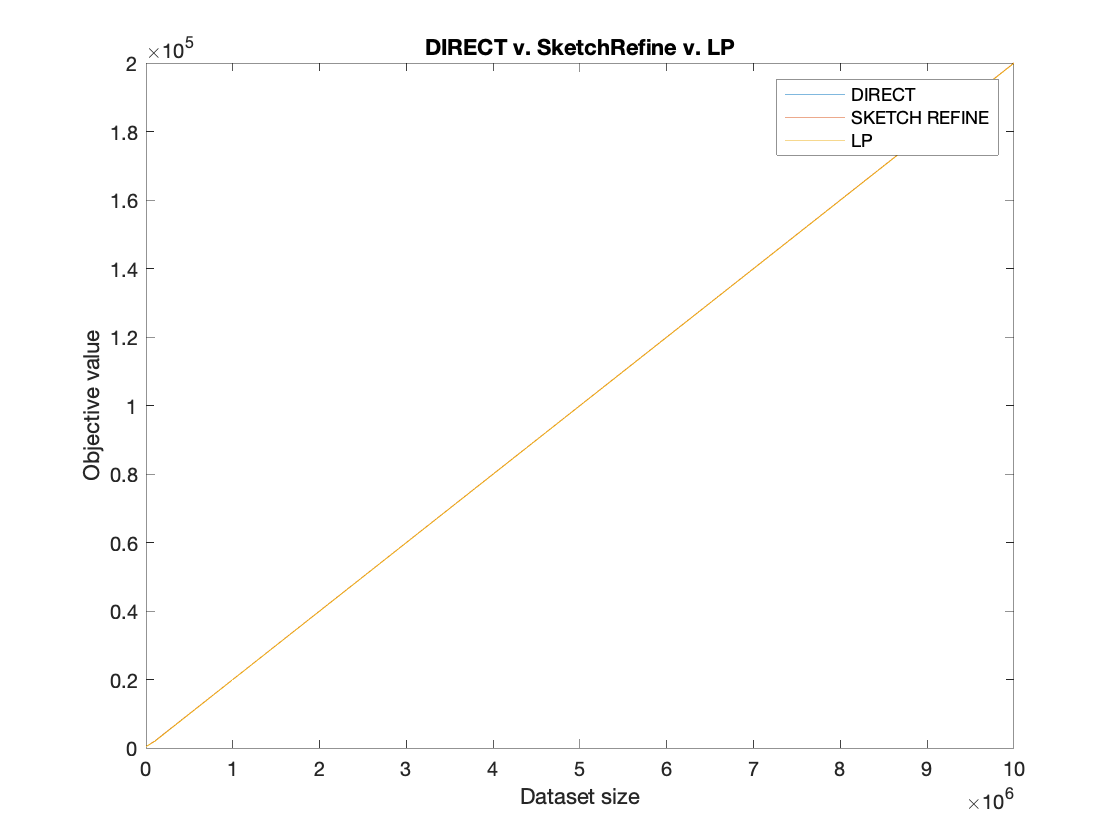
\includegraphics[scale=.4]{8.png}
\caption{DIRECT (ILP) v. SketchRefine v. LP (Objective Value).}
\centering
\end{figure}

In our experiments, we encountered some in-feasible solutions when the constraints were difficult to satisfy. But we never encountered in-feasibility due to long running times. In the paper, however, the Direct (ILP) method failed for some queries [1]. This is due to the size of the dataset involved in the query. Because CPLEX solves the optimization problem while keeping all the data in the memory, it gets over-whelmed with bigger datasets and fails. It also failed for some queries with smaller datasets because the optimization ILP gets too complex for CPLEX to solve and we get an in-feasible solution. SketchRefine is able to get approximated answers even when Direct method fails [1]. Also, the partition size required for SketchRefine has a major effect on its performers. The best partition size, according to experiments, is when the partitions are small and there aren't that many of them [1], which happens when there isn't much variance in the data.
\\

Although the smaller ILP problems take much less time than the single big ILP, SketchRefine has an overhead when it comes to formulating all these smaller ILPs and the backtracking feature. Both methods also spend time accessing data from Postgres, formulating the ILP problems, materializing the tuples from the feasible solution and returning the result. Those times are not included in this paper.
\\

\textit{7.2 sPaQL (Naive v. SummarySearch)}
\\

Since sPaQL paper was published recently, the code hasn't been open sourced yet. Re-implementing the entire code base for Naive and SummarySearch is beyond the scope of this paper. Therefore, results from the paper are presented here. Like PaQL, experiments for sPaQL were performed on Postgres using CPLEX as an optimization solver. Two of the datasets are from real-world applications: the Galaxy dataset [13] with noisy sensor measurements and finance data from Yahoo [14]. The third dataset is TPC-H benchmark containing 117,600 tuples [15].  Figure 11 below shows the end-to-end results of Naive vs. SummarySearch [2]. 
\\

\begin{figure}[h]
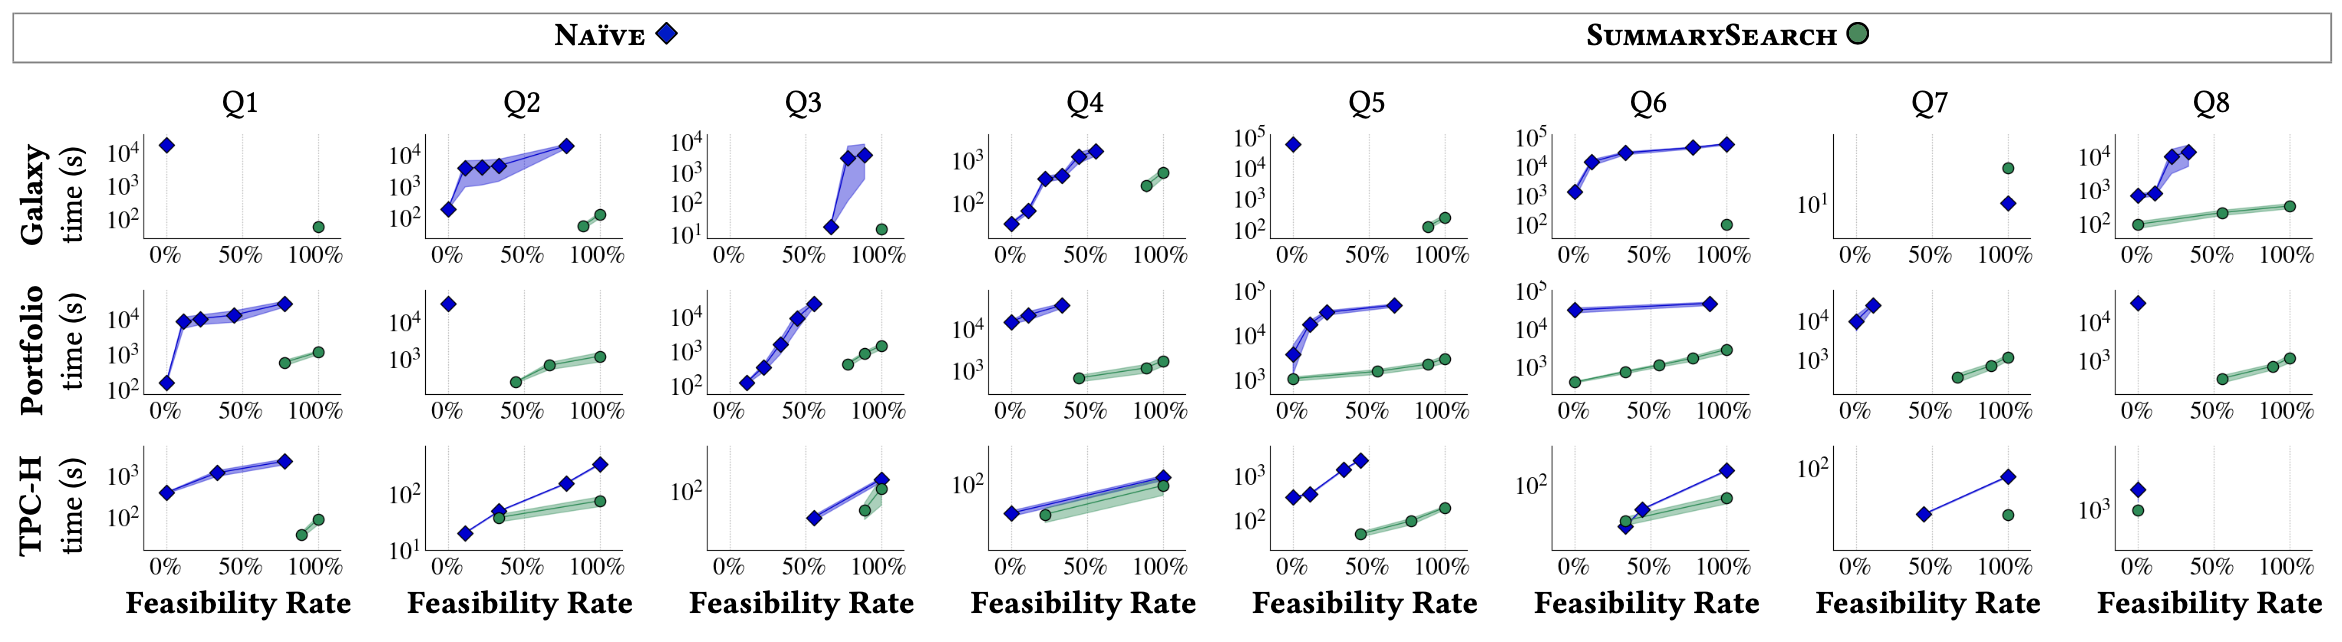
\includegraphics[scale=.4,left]{13.png}
\caption{Naive vs. SummarySearch algorithm. Response time vs. feasibility}
\
\end{figure}
\\
Both methods increase the number of scenarios $M$ to reach feasibility. It can be seen that in many cases, the Naive method just fails to reach 100\% feasibility. SummarySearch, on the other hand, always reaches 100\% feasibility. Also, SummarySearch reaches feasibility much faster than Naive method since its solving much smaller deterministic ILPs using the summaries instead of the entire scenario set. Since the summaries are conservative in nature, SummarySearch reaches feasibility more often even with fewer scenarios. There was one query, however, where SummarySearch was actually slower than the Naive approach (Galaxy - Q7) due to the overhead of generating the summaries and probabilistically unconstrained problem.
\\

As we increase the size of scenario set $M$, the running time of Naive method increases exponentially [2]. SummarySearch, however, is able to find feasible solution even with fewer scenarios [2]. Increasing the size of the summaries slows down the SummarySearch algorithm since as $Z$ goes to the size of scenarios set $M$, SummarySearch essentially degrades into the Naive method. In general, SummarySearch scales well with the size of the dataset [2]. Naive method, on the other hand, times out often as the dataset size goes up. 
\\\\

\textbf{8 Future Work}
\\

Both SketchRefine and SummarySearch are similar techniques as both try to break down the single large ILP problem into many smaller ILP problems that are easier to solve. SketchRefine does this by operating on representative tuples of the dataset based on partitioning it, while SummarySearch operates on the summaries instead of the full scenario set. In that sense, both methods are trying to approximated the original ILP in a smart way using divide-and-conquer techniques. Therefore, it makes sense to generalize and combine both approaches into one. 
\\

One can also extend the Package queries to use open source optimization solvers. Right now, both PaQL and sPaQL are using IBM CPLEX which is a proprietary optimization solver. By using open source solvers, we can look into the black-box and perhaps come up with techniques to solve optimization problem in a better way. For instance, one might look into why LP approximations are not that fast compared to the ILP they are approximating.  Another idea is to model the package queries based on the optimization objective. If its convex, then there is a wide variety of optimization techniques available to solve the problem efficiently. Besides approximating ILPs using LP, one could also use other methods like primal-dual algorithm. 
\\

One limitation of PaQL is that it only supports single relation queries. However, most real-world practical optimization problems involve multiple relations (like Example 1 and 2 in the Introduction above). In order to widen the appeal of solving optimization problems in databases, one must extend PaQL to handle joins of multiple relations. One can also work on handling non-linear constraints and try to work towards expressing different types of optimization problems in the form of package queries.
\\

Similarly, we can extend sPaQL to handle relations spanning multiple tables and integrate it into probabilistic databases. Only single-stage decision making was addressed in the paper [2]. However, in real-world application, we grow less certain as time passes and we accumulate more data. One could integrate the new data with the sPaQL as it is revealed and improve the results of the original package query. On the theoretical side, one could prove convergence results about SummarySearch based upon the number of scenarios it needs. 
\\

\textbf{9 Conclusion}
\\

There have been a lot of advances in Mathematical optimization and database systems are here to stay. It makes sense, therefore, to integrate optimization techniques within databases to allow users, like database analysts, to solve powerful optimization problems while using a familiar language like SQL.
More and more fields are integrating mathematical optimization techniques to take advantage of the faster and improved methods available to solve optimization problems. Databases usually try to stick with conventional techniques of optimizing such as introducing indexes, partitioning, operation re-order and many others such techniques developed over decades. But for certain types of queries, these optimization techniques completely fail to provide a solution and the user has to export the data outside of the database and use optimization solvers. Package queries offer a way to not only declare optimization problems in an easy way by using extension of SQL language, but also to solve them efficiently while never leaving the database system itself.
\\

Package queries come in both deterministic and stochastic flavor. In both cases, the optimization problem is modeled as an Integer Linear Program and solved using off-the-shelf optimization solver. However, it turns out that the approach of directly solving the entire problem in one go often fails in practice. Instead of solving one giant ILP, we break it down into smaller instances of ILP problems that can be solved efficiently. We then combine the results in a smart way to achieve an approximate feasible solution to the original query problem. This solution comes with theoretical guarantees that the objective value is not far from the optimal one. By settling on a sub-optimal but extremely good solution, we buy a lot of performance in return as both SketchRefine [1] and SummarySearch [2] are at least an order of magnitude faster than solving the ILP problem directly. There are many ways to not only improve these methods (parallelization), but also do more research into making optimization tools widely available to the world. To that end, we plan to continue our research combining SketchRefine and SummarySearch into a unified approach to solve ILP problems much faster. 
\\

\bibliographystyle{unsrt}%Used BibTeX style is unsrt
\bibliography{sample}

\begin{enumerate}
  \item [1] M. Brucato, J. F. Beltran, A. Abouzied, and A. Meliou. Scalable package queries in relational database systems. CoRR,abs/1512.03564, 2015.  
  \item [2] M.Brucato, N.Yadav, A.Abouzied, P.J.Haas, and A.Meliou. Stochastic package queries in probabilistic databases. arXiv, 2020.
  \item [3] S. M. Ross. Introduction to Probability Models. Academic Press, 2014.
  \item [4] A. G. Parameswaran, P. Venetis, and H. Garcia-Molina. Recommendation systems with complex constraints: A course recommendation perspective. ACM TOIS, 29(4):1–33, 2011.
  \item [5] A. Meliou and D. Suciu. Tiresias: The database oracle for how-to queries. In SIGMOD, pages 337–348, 2012.
  \item [6] L. Siksnys and T. Pedersen. SolveDB: Integrating Optimization Problem Solvers Into SQL Databases. . In SSDBM (pp. 14:1–14:12). ACM, 2016.
  \item [7] D. P. Williamson and D. B. Shmoys. The design of approximation algorithms. Cambridge University Press, 2011.
  \item [8] Boyd, S., & Vandenberghe, L. (2004). Convex Optimization. Cambridge: Cambridge University Press. doi:10.1017/CBO9780511804441
  \item [9] J. A. Hartigan and M. A. Wong. Algorithm as 136: A k-means clustering algorithm. Applied statistics, pages 100–108, 1979.
  \item [10] L. Kaufman and P. J. Rousseeuw. Finding groups in data: an introduction to cluster analysis, volume 344. John Wiley & Sons,2009.
  \item [11] R. A. Finkel and J. L. Bentley. Quad trees a data structure for retrieval on composite keys. Acta informatica, 4(1):1–9, 1974
  \item [12] J. Luedtke and S. Ahmed. A sample approximation approach for optimization with probabilistic constraints. SIAM Journal on Optimization, 19(2):674–699, 2008.
  \item [13] TheSloanDigitalSkySurvey,datarelease12.http://cas.sdss.org/dr12/.
  \item [14] Yahoo! Finance. http://finance.yahoo.com/.
  \item [15] TPC BenchmarkTMH. http://www.tpc.org/tpch/.
  
\end{enumerate}

\end{document}

